\documentclass[12pt]{article}

\usepackage[margin=2cm]{geometry}
\usepackage{amsmath}
\usepackage{multicol}
\usepackage{nopageno}
\usepackage{SIunits}
\usepackage{graphicx}
\usepackage{enumerate}
\usepackage{enumitem}
%\usepackage{mathabx}
\usepackage{wasysym}


% for making bond drawings
\usepackage{chemfig}
% Global bond settings
\setchemfig{
  atom sep=18pt,               % fixed bond length
  double bond sep=2pt,       % spacing between the two bars
  bond style={line width=0.8pt}
}


% for centering figures on page while in an enumerated/itemized list:
\usepackage{changepage} % in the preamble
\makeatletter
\newenvironment{centerinpage}
  {%
    \par\noindent
    \hspace*{-\@totalleftmargin}% back to page margin (covers all nested list indents)
    \begin{minipage}{\textwidth}% fixed to page width (ignores widened \linewidth)
      \centering
  }
  {%
    \end{minipage}\par
  }
\makeatother

%%%%%%%%%%%%%%%%%%%%%%%%%%%%%%%%%%%%%%%%%%%%%%%%%%%%%
% For putting links in the document (both to sections and hyperlinks)
\usepackage{hyperref}
\usepackage{url}
\hypersetup{
    colorlinks=true,     % false: boxed links; true: colored links
    linkcolor=red,       % color of internal links
    citecolor=blue,      % color of links to bibliography
    filecolor=blue,      % color of file links
    urlcolor=blue        % color of external links
}
% below, use \url{http://www.nytimes.com} (they will be urlcolor)
%%%%%%%%%%%%%%%%%%%%%%%%%%%%%%%%%%%%%%%%%%%%%%%%%%%%%


%%%%%%%%%%%%%%%%%%%%%%%%%%%%%%%%%%%%%%%%%%%%%%%%%%%%%
% for the events page boxes

% boxed regions
\usepackage{tcolorbox}
\tcbuselibrary{skins,breakable}

% fonts & spacing
\usepackage{lmodern}
\usepackage{microtype}
\usepackage{calc}


% small helper macros (adjust these)
\newcommand{\boxheight}{4.2cm}   % height for each event box
\newcommand{\boxfont}{\scriptsize} % change to \tiny or \footnotesize as desired
\newcommand{\linelen}{0.95\linewidth} % timeline line length

%%%%%%%%%%%%%%%%%%%%%%%%%%%%%%%%%%%%%%%%%%%%%%%%%%%%%
\newcommand{\rmd}{\ensuremath{{\rm d}}}
%\newcommand{\vv}[1]{\ensuremath{\vec{#1}}}
\newcommand{\vv}[1]{\ensuremath{\mathbf{#1}}}
\newcommand{\ee}[1]{\ensuremath{\mathbf{e}_{#1}}}
%%%%%%%%%%%%%%%%%%%%%%%%%%%%%%%%%%%%%%%%%%%%%%%%%%%%%



\begin{document}

\begin{center}
{\Large Greenhouse Effect: Infrared Absorption Spectrum}
\end{center}
%%%%%%%%%%%%%%%%%%%%%%%%%%%%%%%%%%%%%%%%%%%%%%%%
%%%%%%%%%%%%%      overview         %%%%%%%%%%%%%%%%%%%%%
%%%%%%%%%%%%%%%%%%%%%%%%%%%%%%%%%%%%%%%%%%%%%%%%

\noindent In our work over the last week, we investigated how the structure of molcules determines their potential to act as greenhouse gases (absorbing the infrared radiation of the Earth's surface). We found that:
	%
	\begin{quote}
	a molecule can absorb infrared photons if there is some oscillation of the molecule (vibration, bending, rotation) that causes its net electric dipole moment to change
	\end{quote}
If such an oscillation exists, then passing infrared photons will be absorbed by the molecule, and the energy they deliver will ``excite'' the oscillation.  We saw that a ``changing dipole moment'' is possible if one or both of the following is true:
		%
		\begin{enumerate}[label=(\roman*)]
		\item The molecule has a net electric dipole moment (when relaxed), which can be altered by the electric field of a photon of electromagnetic radiation.
		\item The molecule has a net zero electric dipole moment when relaxed, but some non-relaxed configurations have a non-zero dipole moment; these oscillations --- accompanied by a changing dipole moment --- can be induced by infrared photons.
		\end{enumerate}
		%
	Both of these can occur together (e.g., in the water molecule), or just one (e.g., carbon dioxide, $\text{CO}_2$, and methane, $\text{CH}_4$, are both symmetric molecules and so they have zero net dipole moment; but when their bonds are stretched asymmetrically, they do have a dipole moment).\\[-6pt]

\noindent Today we will investigate how the absorption of infrared photons in Earth's atmosphere causes a loss of energy reaching space, which is observed as so-called {\bf absorption lines} in the blackbody spectrum.  The key ideas of absorption are these:
	%
	\begin{itemize}
	\item The energy of light is carried in photons, which are packets of light of a single color (a single wavelength or frequency).  The amount of energy in a single photon is given by the equation:
		%
		\begin{equation*}
		E = h f = h \frac{c}{\lambda}
		\end{equation*}
		%
	where $h = \unit{6.6\times10^{-34}}{\meter^2 \kilo\gram / \second}$ is called Planck's constant, $f$ is frequency, and $\lambda$ is wavelength.  This means that a single \unit{6}{\micro\meter} wavelength photon has just  $33 \times 10^{-19}$ Joules of energy (33 ``zeptojoules''!).  To simplify our calculations, we will use this easy conversion between frequency in terahertz ($1\unit{\tera\hertz} = \unit{10^{12}}{\hertz}$) and wavelength in micrometers:
		%
		\begin{equation*}
		f \,[\text{THz}] = \frac{300}{\lambda \, [\micro \text{m}]}
		\end{equation*}
	\item A type of ``oscillation'' is called a ``mode'' or ``vibratory state'' of the molecule.  Its excitation has a certain fundamental energy associated to it, and, if accompanied by a changing electric dipole, it will be excited by photons of a specific frequency/wavelength (see Figure 1 and Question 2; in Figure 1 these wavelengths are labeled by ``$\nu$'' instead of ``$\lambda$'' for some reason).
	\item Combinations of multiple oscillations can also occur. The sum of their excitation energies can then be associated to a single photon frequency that can excite the combination.  A special case of this is a ``double excitation'' (or triple, \ldots) of a single oscillation type; so, if $f$ is an excitation frequency, than $2f$ is also an excitation frequency. (See Question 3).
	\end{itemize}
	%

\newpage
%%%%%%%%%%%%%%%%%%%%%%%%%%%%%%%%%%%%%%%%%%%%%%%%
%%%%%%%%%%%%%      questions         %%%%%%%%%%%%%%%%%%%%%
%%%%%%%%%%%%%%%%%%%%%%%%%%%%%%%%%%%%%%%%%%%%%%%%

\begin{enumerate}

\item {\bf Electric dipoles and absorption} For each of the three greenhouse gas molecules shown in Figure 1, complete the following steps:
	%
	\begin{itemize}
	\item Draw the structure for yourself, reminding yourself why it looks as it does, using our ``chemistry'' work in the previous discussion\footnote{We didn't consider Ozone ($\text{O}_3$) before.  To figure out its Lewis dot structure, first consider the {\em total number} of valence electrons it has across all three atoms. Then assign these electrons to the  three-atom structure in such a way that each atom gets eight electrons (either in lone pairs or shared).  You should find a single bond and a double bond.}.
	\item On one picture of the molecule, draw an electric dipole vector along each bond.  If there are identical types of bonds (e.g., the two carbon to oxygen bonds in $\text{C}\text{O}_2$) then they should have identical length vectors.  Using the rules of vector addition that we learned on the previous discussion, determine if the resting molecule has a net dipole moment or a zero dipole moment.
	\item Now consider the three ``vibratory states'' (vibration along bonds, or bending of the molecule) shown in Figure 1.  Explain each of these oscillations with a {\em sequence of pictures}, showing how the structure changes over time, periodically.
	\item Under the oscillations shown in the previous step, will the net dipole moment change?  Check your answers\footnote{The answer is ``yes'' if there is a wavelength assigned to the oscillation in Figure 1 (it is yes for eight of the nine).} using the information given in Figure 1.
	\end{itemize}

\vspace{1cm}

\item {\bf Drawing absorption spectra on blackbody radiation curves} 
	%
	\begin{enumerate}
	\item Recall from Week Four's discussion how we drew blackbody curves on log-log paper.  Sketch the Earth's blackbody spectrum on the log-log paper provided, assuming an average temperature of $T_\text{Earth} = \unit{288}{\kelvin} = 15\degree\text{C} = 60\degree\text{F}$. Remember this involves finding: the wavelength of the peak, $\lambda_\text{peak}$; the maximum value of the spectral flux; and wavelength positions ($\lambda_\text{peak}/2$ and $3 \lambda_\text{peak}$) of the ``$\frac{\text{peak}}{10}$'' values of spectral flux .  Calculate all values first before setting the scale on your axes, so that you can fill the whole page. The horizontal axis should be the wavelength in units of  micrometers, $\unit{1}{\micro\meter} = \unit{10^{-6}}{\meter}$.
	\item For each of the three greenhouse gases in Figure 1, find the wavelength of infrared radiation that excites each mode (these are given in Figure 1).  Draw a dot on your blackbody curve for each of these (you should have 8 dots) and put a nearby label  with the name of the gas and type of vibration.
	\item Consider Figures 2 and 3.  Find the same eight infrared absorption wavelengths on one or both of these plots and mark them with a vertical line across all sub-graphs.  Do these lines make sense based on the information being presented in the figure? Explain. 
	\item Figure 2 shows that most of these lines absorb almost 100\% of outgoing infrared light at their peak wavelength.  Explain how this is seen in the graph(s).  Then, for a few of the wavelengths (two or three), identify the wavelength values, above and below the wavelength of the center of the line, where the absorption falls to 10\%.
	\item Using those 10\% absorption wavelengths, draw approximate absorption ``valleys'' on your own blackbody curve.  Draw two dots for the values you found, remembering that dropping by 10\% means going down by one major tick mark on a logarithmic axis.
	\end{enumerate}
	
\newpage

\item {\bf Additional absorption lines}  You might have noticed that there are many absorption lines (places where infrared light is strongly absorbed) shown in Figure 2 that were not accounted for in the eight fundamental absorption lines for water, carbon dioxide and ozone.  Many of the lines can be determined from {\em multiple-oscillation excitations} whose total energy is provided by a single photon corresponding to that total energy value.  This can be double- or triple-excitations (etc) of a single oscillation mode, where a single photon puts twice or three times the amount of energy into the oscillation. Or, it can be a true multiple-oscillation mode (e.g., a combination of bending and stretching) that is excited by a single photon with energy equal to the sum of the constituent oscillation energies.\\[-6pt]

\noindent Let's start with water (we'll come back to $\text{CO}_2$ and ozone if we have time) and complete the following steps.
	%
	\begin{enumerate}
	\item Calculate the frequency (in terahertz, THz) for each vibratory state from its wavelength in micrometers\footnote{See the simple conversion equation on the first page of this discussion. Unhelpfully, the wavelengths in Figure 1 are labeled with the Greek letter ``nu'' instead of ``lambda'': $\nu$ is given in micrometers, so just think of it as $\lambda$. }.  Call these $f_1$, $f_2$, and $f_3$, corresponding to the $\lambda$ values in Figure 1.
	\item Make a table with columns: $[n_1, n_2, n_3, \text{sum-of-freq}\footnote{The sum of the frequencies will be proportional to the energy of the combined oscillation because of $E = h f$, as described on the first page. So the actual procedure should be (i) Calculate the frequency of the vibratory state from its wavelength. (ii) Calculate the energy of the vibratory state from its frequency, using $E = hf$. (iii) Sum the energies of the combined vibratory states. (iv) Calculating the frequency associated to that combined energy using $E_\text{tot} = h f_\text{tot}$. (v) Calculate the wavelength associated to $f_\text{tot}$.  But because of that proportionality between energy and frequency we can skip steps (ii)-(iv)!}, \lambda]$.  
		%
		\begin{enumerate}
		\item You can fill in the first row of your table with $n_1=1$,  $n_2=0$, and $n_3=0$ to represent the first vibratory state; then the ``sum-of-freq' will just be the $f_1$ value and the wavelength  will be that of the first vibratory state.  Do the same in the next two rows, using the information for the second and third vibratory states. These first three rows correspond to the modes we already found in the absorption lines of Figures 2 and 3.  
		\item Now, in the fourth row, consider the multiple-oscillation case of combined ``symmetric stretching'' plus ``bending.'' You will put $ (n_1, n_2, n_3) = (1, 1, 0)$ for the n values, and the ``sum-of-freq'' column will show ``$f_1 + f_2 = \ldots$''.  Finally convert that total frequency value to a wavelength in micrometers.  
		\item Complete some more rows either by combinations of different oscillations, or multiple excitations of the same oscillations, e.g., $(n_1, n_2, n_3) = (2, 0, 0)$.
		\end{enumerate}
		%
	\item For each row in your table, identify the locations of the absorption lines on the water vapor graph within Figure 2.  Did you find all of them?  Are there any that you predicted that you did not find?
	\item Why are there two carbon dioxide absorption lines between \unit{2}{\micro\meter} and \unit{3}{\micro\meter}?  What are their exact wavelength value?
	\end{enumerate}

\end{enumerate}
\newpage
%%%%%%%%%%%%%%%%%%%%%%%%%%%%%%%%%%%%%%%%%%%%%%%%%%%%
%%%%%%%%%%                    greenhouse  molecules                                 %%%%%%%%%%%%%%
%%%%%%%%%%%%%%%%%%%%%%%%%%%%%%%%%%%%%%%%%%%%%%%%%%%%

\begin{figure}[h]
\begin{center}
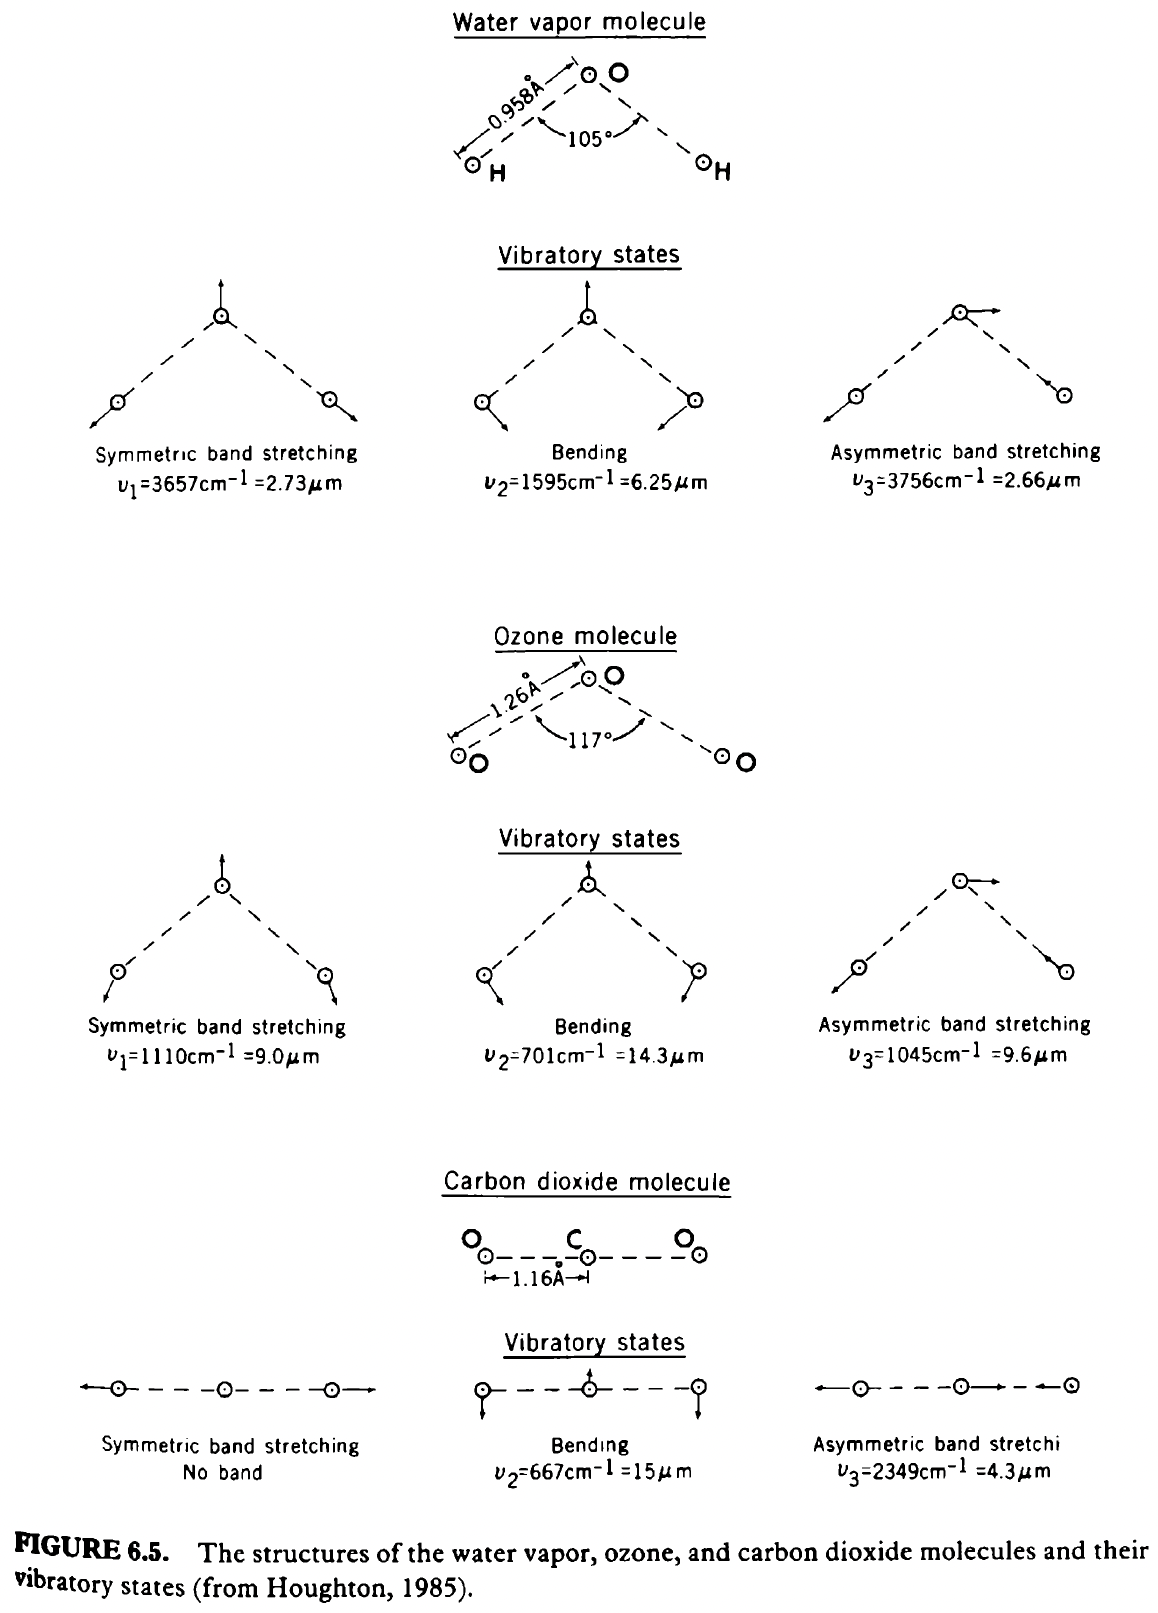
\includegraphics[width=0.9\textwidth]{images/peixoto_fig6-5_structure-water-ozone-co2.png}
\end{center}
\caption{
From Peixoto textbook
}
\end{figure}

\newpage
%%%%%%%%%%%%%%%%%%%%%%%%%%%%%%%%%%%%%%%%%%%%%%%%%%%%
%%%%%%%%%%                    absorption  spectrum (rohde)                                 %%%%%%%%%%%%%%
%%%%%%%%%%%%%%%%%%%%%%%%%%%%%%%%%%%%%%%%%%%%%%%%%%%%

\begin{figure}[h]
\begin{center}
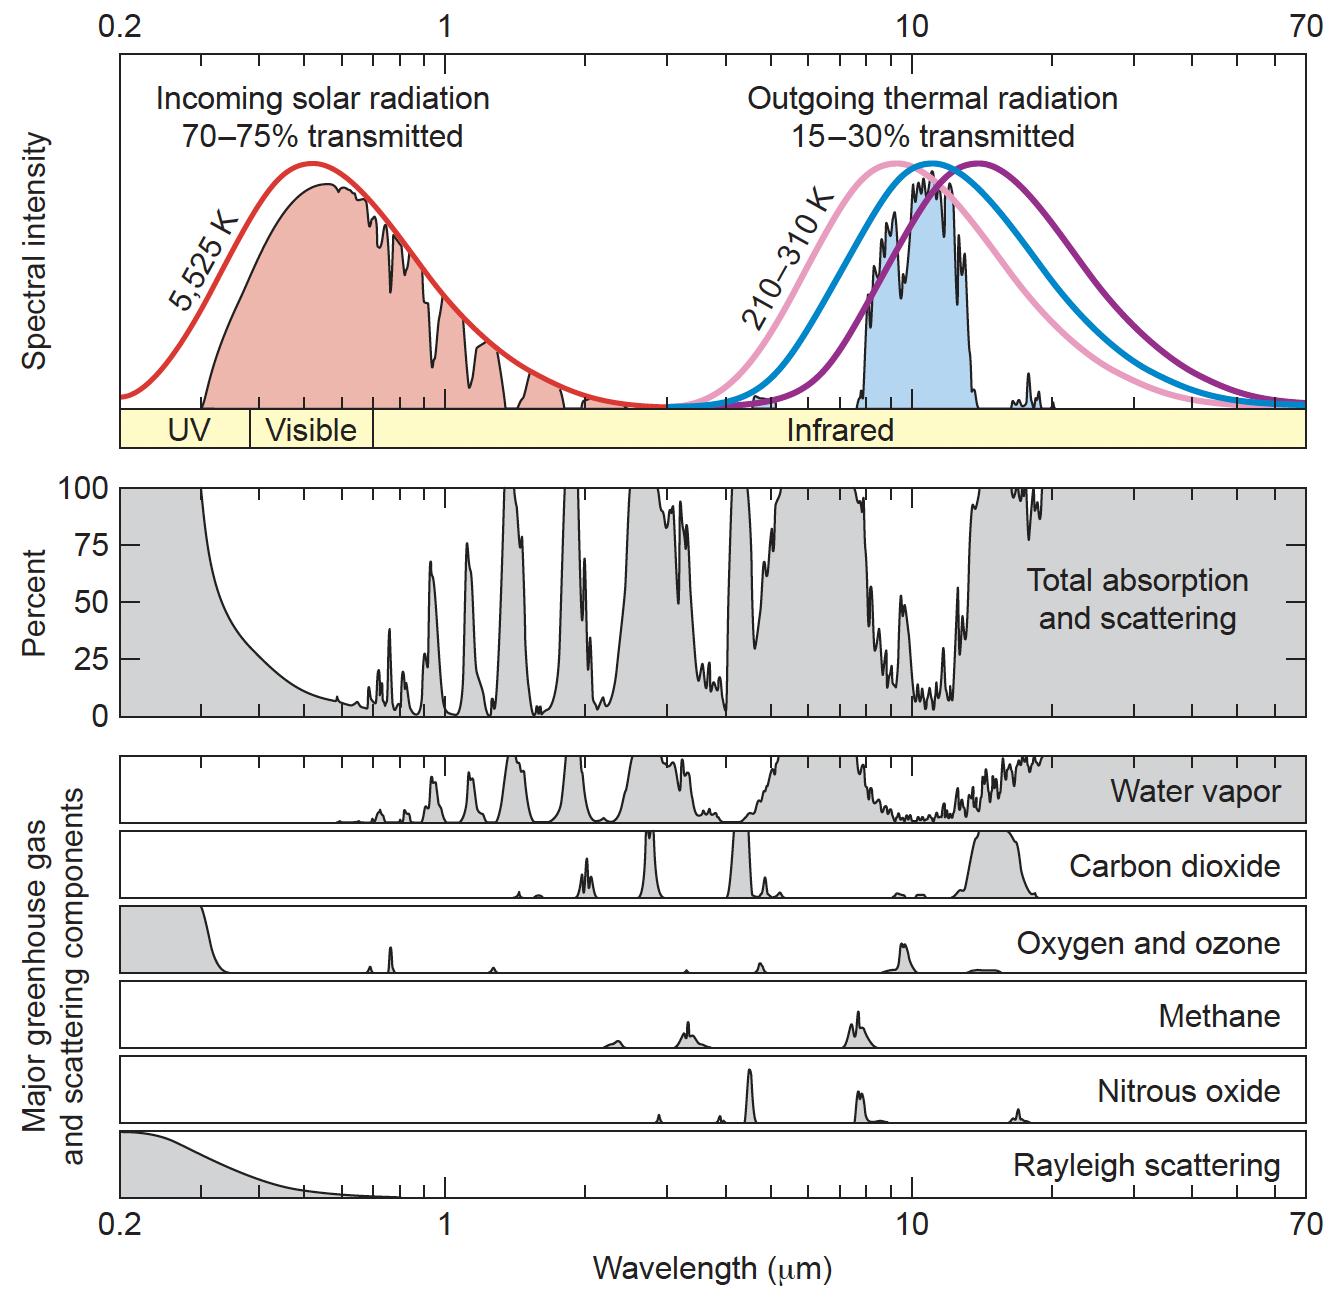
\includegraphics[width=\textwidth]{images/atmospheric-absorption-transmission_rohde_mathez-textbook_no-caption.png}
\end{center}
\caption{
Figure by Rohde, from Mathez textbook
}
\end{figure}

\newpage
%%%%%%%%%%%%%%%%%%%%%%%%%%%%%%%%%%%%%%%%%%%%%%%%%%%%
%%%%%%%%%%                  absorption spectrum on BB                                 %%%%%%%%%%%%%%
%%%%%%%%%%%%%%%%%%%%%%%%%%%%%%%%%%%%%%%%%%%%%%%%%%%%

\begin{figure}[h]
\begin{center}
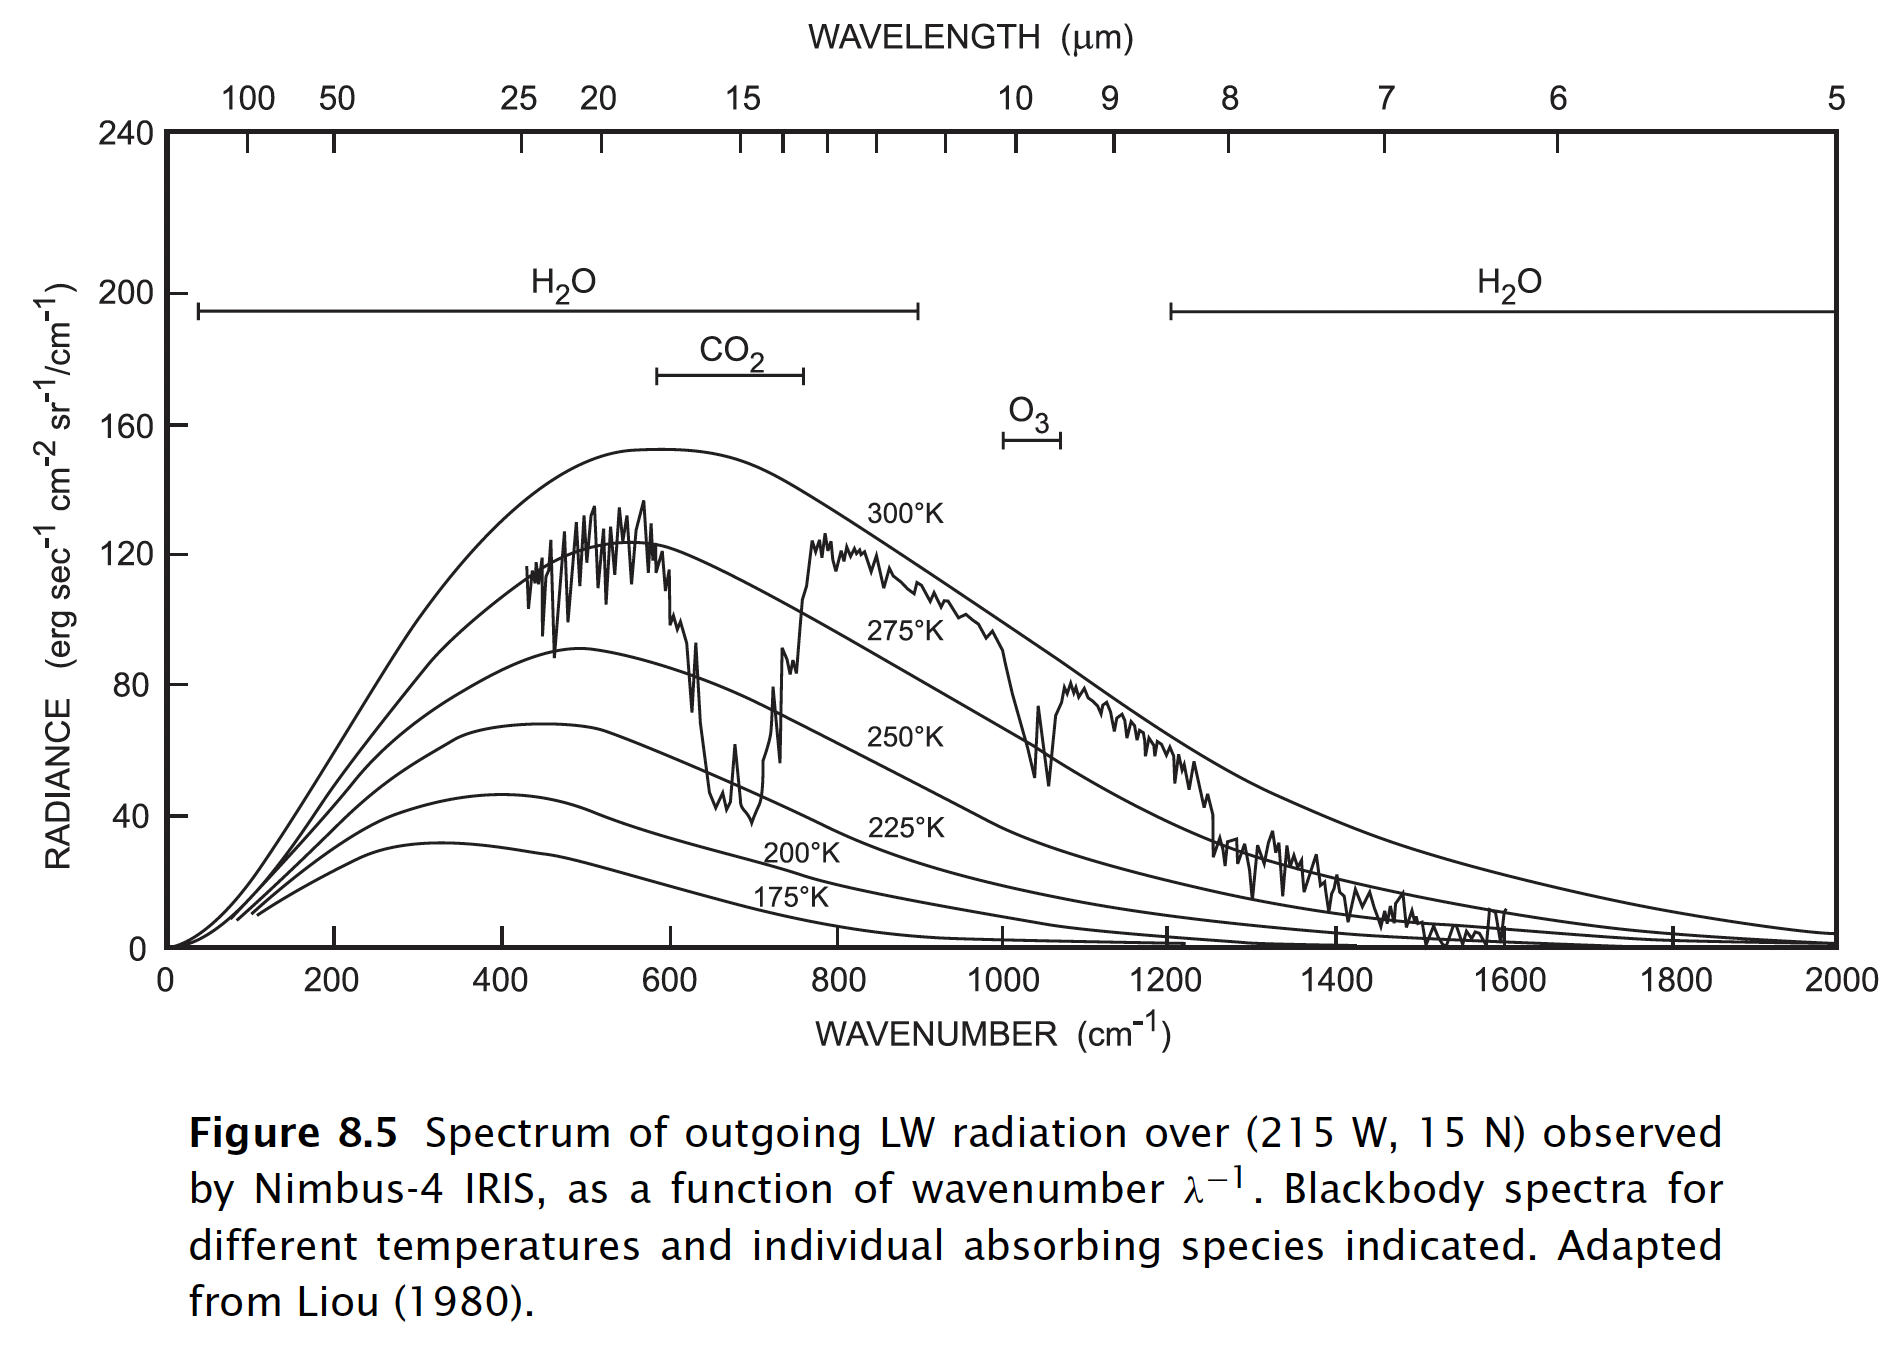
\includegraphics[width=\textwidth]{images/salby_fig8-5_outgoing-infrared-lines.png}
\end{center}
\caption{
From Salby textbook
}
\end{figure}



%%%%%%%%%%%%%%%%%%%%%%%%%%%%%%%%%%%%%%%%%%%%%%%%%%%%
%%%%%%%%%%                                  References                                %%%%%%%%%%%%%%%%
%%%%%%%%%%%%%%%%%%%%%%%%%%%%%%%%%%%%%%%%%%%%%%%%%%%%
%\noindent {\bf Data Sources}: 



\end{document}
